\section{Transitioning to Three Dimensions}
The move to 3D was slow, the jump from \emph{pygame} to a full blown physics simulation was a big leap and it came with its problems.

\subsection{CoppeliaSim and RLBench}

CoppeliaSim is a mostly open source simulation program that provides full access to its features through an educational license and RLBench is an in-house (Imperial) tool adapted to plug into CoppeliaSim through its python API interface (PyRep \cite{}) \todo{cite pyrep}. 

There are many tutorials online to help learn how CoppeliaSim operates and designing some scenes \todo[color=green]{maybe cite some stuff here, not necessary}. However, RLBench is a harder beast to tame. Although the system is very smart and eliminates a lot of the manual work needed to be done before starting experimentation, it was now slightly out of date and I had many issues setting it up on my system.

\subsection{Environment Issues}\todo{entire section needs a reread and structuring}
One of the first large-scale issues I'd face in this project came here, quite early in its lifespan. I would soon learn robotics development is mostly done on Linux based machines and the journey to getting everything working would be quite long.

\subsubsection{Windows Setup}
I do most development work on Windows and WSL (Windows Subsystem for Linux) \cite{} and expecting this project to be fairly memory and graphic power hungry I though I'd setup everything on the Windows side. This caused a few issues with PyRep, this was becuase PyRep firstly expected to be running on Linux, and RLBench was having issues working.

\subsubsection{WSL Setup}
I thought this wouldn't be a problem, as WSL version 2 has been pretty good with GUI applications running on Linux and thought I could run Coppelia on there and still access any displays I might need. The translation layer between the operating systems might cause some slowing but there shouldn't be any major issues issue. Upon configuring everything as the installation guide suggested in RLBench and PyRep repositories. I had few issues linking object files downloaded with CoppeliaSim into the PyRep layer had some issues. After spending a lot of time researching issues, and coming across some online threads with similar issues (in different applications, so nothing was immediately applicable) I decided WSL must have been the problem and decided to move onto the next logical step.
 
\subsubsection{Linux Virtual Machine}
I had previously used Ubuntu a lot and even my WSL instance was running Ubuntu. As RLBench suggested Debian based systems, assuming they also developed it in Ubuntu, I created a Virtual Machine running it. After the entire setup process, I was finally able to get the instance running and finally managed to run one of the examples that gets downloaded when installing RLBench.

However, I got hit by another issues fairly quickly, the rendering of Virtual Box was definitely going through some sort of translation through Windows and then the GPU (not even sure, maybe it was all CPU rendered) however, everything was extremely sluggish, and running the non-primitive examples even crashed my virtual machine instances a few times. At this point I realised I had to settle for the real deal and got to partitioning by storage drive.

\subsubsection{Dual Booting}
I had some issues partitioning the drive Windows was already installed, as it had making that its home and spread all around the disk. I currently had no ways of backing up my data and erasing my disk to completely wipe then partitioning before installing windows again. So, I ripped a spare drive I had in my old laptop and booted Linux form there. After running through the same setup steps, I was finally properly running RLBench. With one caveat, CoppeliaSim constantly complained that I was missing some video encoding binaries, though seemed to work perfectly fine; even when I fixed the binaries it would work but every once in a while pop up saying I was missing them. There were other small annoyances like this throughout the entirety of the experimentation but at least now it was working.

\subsubsection{Campus Machines}
I knew that a solution to all of my problems might have been using a machine at the labs. I thought an issue with that may have been that RLBench requests a lot of binary linking and editing which might have required and the troubleshooting wouldn't be as easy as doing it on my machine. Which could be resolved if I requested a machine to use, but I though my personal machine had the appropriate powerful hardware for a machine learning project and wanted to use that. So jumping through all these steps tool about an entire week, but was well worth it at the end.


\subsection{Usability Issues}
One of the major instability issues I had was because RLBench is about 5 years old now and CoppeliaSim has moved on in some parts, and I was not able to get exactly the same version of the simulator they had as well as exactly the same version of the libraries used when developing RLBench.

\subsubsection{RLBench Codebase}
As I started using RLBench other issues started popping up, PyRep was randomly failing calls to CoppeliaSim due to errors raised in RLBench due to unexpected types and hitting exceptions such as \emph{``Should not be here''} which was especially frustrating. However, the solution was simple. Entirety of the RLBench source code is accessible, so instead of downloading it as a package I forked the repo and started fixing any issues as they started arising. Once trivial issues were getting fixed I also started using CoppeliaSim to make mockup tasks (to be outlined in the future \todo{linking!}) and create networks that would use the simulation to train.

\todo{mention RLBench and accompanying API PyRep are written for Coppelia v4.1.0, which is now almost 5 years old (https://manual.coppeliarobotics.com/en/versionInfo.htm), updating coppelia had issues with PyRep not working}

Around the time I started training some primitive models and learning more about these tools, I started hitting weirder errors, like the simulator constantly crashing, getting unexpected observation results (cameras such as overhead cameras  missing their input) and other weird issues. Spending even more time combing though some of the \emph{enourmous} codebase I would sometimes find issues to fix them, but it would routinely break some of the package binaries I had linked and just stop working with no way to reason or figure out how to fix it. At this point I decided to try some other tools.

\todo{add picture of the missing libraries thingy}

\subsubsection{PyBullet}\todo{add pybullet reference}
The first option was PyBullet, an open-source Python module for simulation, it wraps the C API of Bullet and provides a completely customisable simulation experience. Though, the GUI experience is lacking and almost everything is controller through this C API. 
Following some rough tutorials and combing through the manual for the module, I was able to put together fairly simple graphics, and shapes to start creating some tasks. Although, I came to a halting realisation soon after. Which was that without a complete robot learning suite at my disposal I would need to figure out a lot of the systems from scratch. Such as camera placements and movement systems, seamless task creation and linking, environment management and so on.


\subsection{Toolset Dilemma}\todo{needs a total rewrite this is more of a plan/rough draft}

Faced a lot of issues with RlBench, however, the time I spent on it was too long and learnt how to fix any issues when they came up. It also provided niceties like requesting demos and wiring environment and tasks fairly seamlessly.

On the other hand, PyBullet was customisable and I think overall ran better, coppeliasim (and especially my installation had a few issues which i couldnt seem to fix) but a lot of the ground work done by rlbench I would need to redo. 

So the main dilemma was, should I be wasting time making a comprehensive suite to fit my needs early on in the project and then cancontinue with the premise of the task, or stick with rlbench and solve issues as they arose. Once I fixed a lot of the OS dependent errors, newer versions of coppelia was for some reason not very happy with newer Ubuntu versions, I decided to stick with rlbench, and hoping any issue arising from this point on shouldn't be a system breaking one, and I was familiar enough with the rlbench codebase to at least attempt to fix anything at this point. So I went back to square one and got the work on rlbench.



I didn't do any meaningful work in terms of experimenting with learning or robots, but spent majority of my time setting up RLBench (quite tricky OS requirements and problems) and playing around to get myself familiar with the software. \todo{following to be deleted}



\section{First Steps in 3D: Reaching Task}
Landing back on RLBench and solving most of the issues, first steps were to create some 3d environments and tasks to test capabilities of simple policies on tasks that progressively get more difficult. So, the very first step was to directly translate the 2D task I played with earlier in \ref{subsec:ew-2d-problem}. This mean that I could create a simple reaching task, which not will happen in a 3D environment, with realistic physics simulation

\subsection{Creating the Task}
As discussed before, RLBench provides an intuitive method for quickly creating and validating tasks. \todo{link the tutoirals and the videeos maybe?}. Following the tutorials provided by the creator of RLBench and other resources online on CoppeliaSim \todo{link some copsim manuals or information here.} I could now create tasks for my use case.

Tasks are created using the \emph{`task builder'} CLI, which is a user facing interface that talks to the PyRep API which in turn controls CoppeliaSim. This allows the user to use GUI elements within the simulator to create objects, boundaries as well as edit their properties while observing what they look like in different camera view layers. Then to create scene wirings; the automatically created \verb|Task| class is used, where \emph{initialisation}, \emph{episode step} and other task related systems can be created for the scene object to then use to create demonstrations and train robot policies. See Figure \ref{fig:task-builder}.

\begin{figure}[htbp]
  \begin{subfigure}{0.48\linewidth}
    \centering
    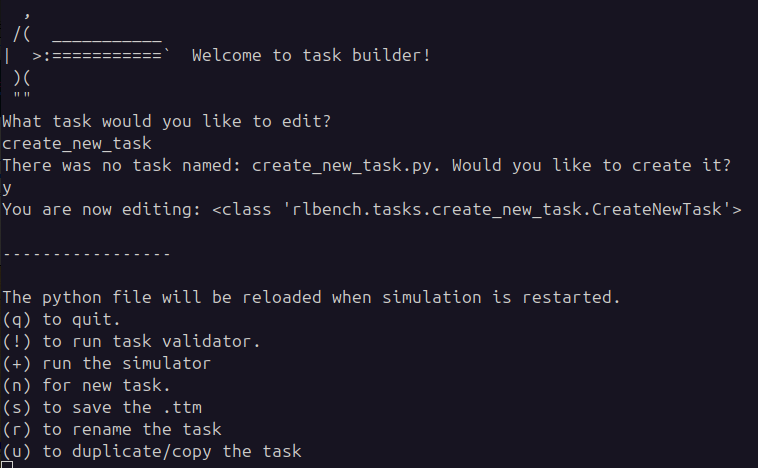
\includegraphics[width=\linewidth]{assets/early-work/task-builder-cli-1.png}      \caption{Task builder CLI: creating a new task}
  \end{subfigure}%
  \hfill
  \begin{subfigure}{0.48\textwidth}
    \centering
    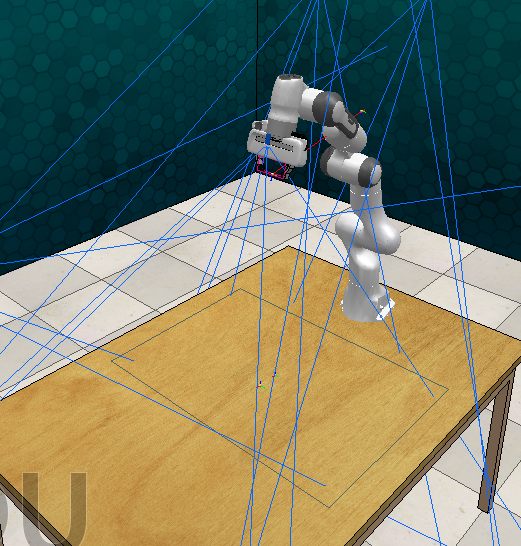
\includegraphics[width=\linewidth]{assets/early-work/task-builder-scene.png}
    \caption{Simulator: Graphical view of the new task}
  \end{subfigure}%
  
  \vspace{0.5cm}
  
  \begin{subfigure}{0.48\linewidth}
    \centering
    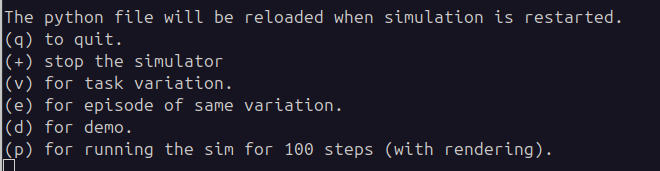
\includegraphics[width=\linewidth]{assets/early-work/task-builder-cli-2.png}
    \caption{Task builder CLI: running the simulator on new task}
  \end{subfigure}
  \hfill
  \begin{subfigure}{0.48\textwidth}
    \centering
    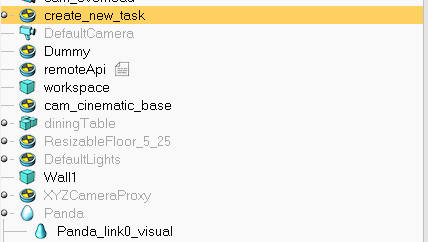
\includegraphics[width=\linewidth]{assets/early-work/task-builder-scene-hierarchy.png}
    \caption{Simulator: Scene Hierarchy of the objects in the new task}
  \end{subfigure}
  \caption{Creating a new task with `task builder'}\label{fig:task-builder}
\end{figure}\


The task I created is simple, see Figure \ref{fig:reach-no-obs}. I decided to use the \emph{Panda arm}, as that seemed to be standard and more importantly immediately supported by RLBench. It has 7 Degrees of Freedom (DoF) and a gripper -so the action space is a 8 dimensional vector. Then a red spherical target, which is not tangible, in the simulation it will be visually rendered but the arm will not collide or interact physically with it. Finally, added a proximity sensor to the target (which is not visually rendered) so the task can be immediately classified as completed by the system.



% //NOTE: relative paths for images, maybe add submodule once project is finished
\begin{figure}[htbp]
  \begin{subfigure}{0.48\linewidth}
    \centering
    \includegraphics[scale=0.4]{../fyp/assets/task-pics/reach-no-obs/random-front.png}      
    \caption{Front View}
  \end{subfigure}%
  \hfill
  \begin{subfigure}{0.48\linewidth}
    \centering
    \includegraphics[scale=0.4]{../fyp/assets/task-pics/reach-no-obs/random-top.png}
    \caption{Top View}
  \end{subfigure}
  \vspace{0.5em}
  \begin{subfigure}{1\linewidth}
    \centering
    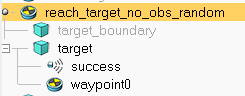
\includegraphics[scale=0.5]{assets/early-work/random-scene-hierarchy.png}
    \caption{Scene Hierarchy}\label{fig:reach-no-obs-hierarchy}
  \end{subfigure}%
  \caption{Reaching Task with no obstacles}\label{fig:reach-no-obs}
\end{figure}

\subsection{Creating a Policy}

The next step was to create a policy network. As I am mainly working on imitation learning from demonstrations provided by the system, my network needs to be able to ingest these demonstrations and generate actions in the action space of the robot. \par

\fbox{  
  \begin{minipage}{\linewidth}
    \textbf{Aside on RlBench Demonstrations} \par
    Demonstrations are provided encapsulated in a \emph{Demo} class and contain a series of observations (belonging to a class \emph{Observation}). These include state information of the robot and the environment, containing information like the observations of the set cameras and sensors; which need to be configured when the environment is started. This modular approach means I can collect demonstrations, then selectively choose what to use, like ignore a camera or a sensor. \par 
    Demonstrations are created following waypoints. PyRep expects  \emph{Dummy} objects within the scene called ``waypointX'' where sequence number of the waypoint starting from $0$. Then he demonstration engine calculates trajectories to these waypoints in sequence. For example, in Figure \ref{fig:reach-no-obs-hierarchy}, we have `waypoint0' within the target, for which a trajectory will be calculated from the tip of the robot gripper.
  \end{minipage}
}

\noindent By default the demonstrations -which I will refer to as ``demos'' from now on- and specifically the cameras pre-placed in the scene, produce images of resolution $128 \times 128$ pixels. I binned this down to $64 \times 64$. This comes in handy as I can keep the processing power low and can adapt the policy for higher resolution cameras by scaling it up later on. Therefore, I created a simple network following this architecture outlined in Figure \ref{fig:policy-arch}. The full code can be found in \todo{add the code of the network to appendix}.

\begin{figure}[h]
  \centering
  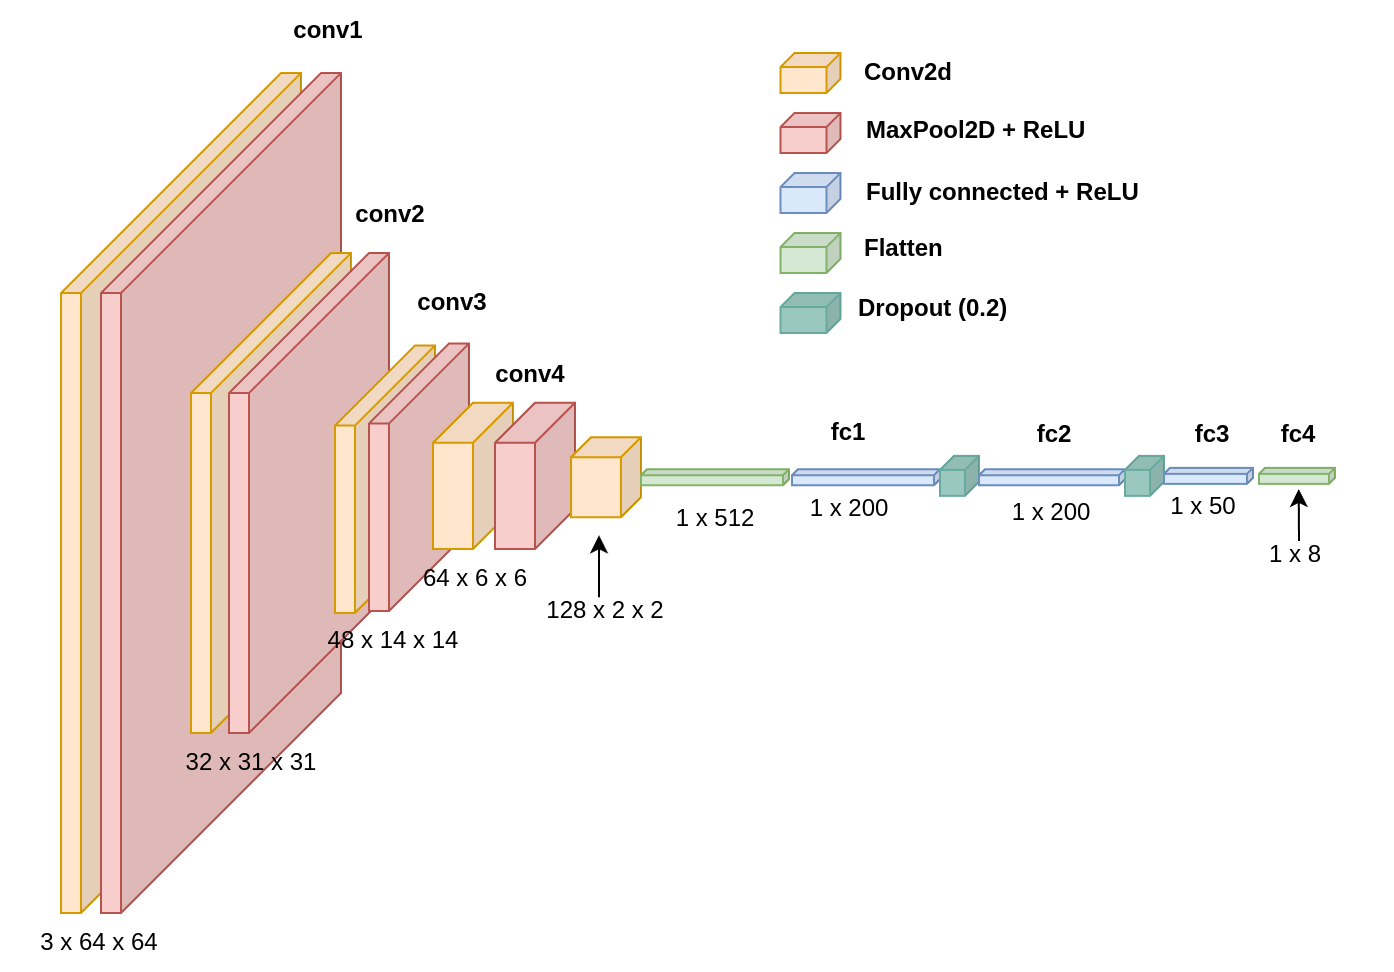
\includegraphics[width=0.8\textwidth]{assets/early-work/cnn-encoder-policy-head.png}
  \caption{Simple Policy Network Architecture}\label{fig:policy-arch}
\end{figure}\todo{ius the quality bad? reuload or reexport the xmml is in assets}


\subsubsection{Tuning the Policy}\todo{can remove not sure??s}

\subsubsection{Policy Improvements}
\todo{maybe do some lr scheduling and data processing for the images for generalisation  and mention the shuffling etc of the data and that it doesn't change much}



\subsubsection{Testing Visual Limits}\todo[color=red]{not sure about these to be honest, maybe remove these??}


conditions are not always ideal, so wanted to do some quick checks to get concrete results on how the agent behaves when the target is placed on the fringes of its field of vision. So created the three tasks shown in Figure \ref{fig:no-obs-3-views}.

\begin{figure}[htbp]
  \begin{subfigure}{0.3\linewidth}
    \centering
    
\includegraphics[scale=0.4]{../fyp/assets/demo-trials-no_obs/tasks/static-tasks-camera/initial-obs-side_l.png}      
    \caption{Left Side}
  \end{subfigure}
  \hfill
  \begin{subfigure}{0.3\textwidth}
    \centering
    
\includegraphics[scale=0.4]{../fyp/assets/demo-trials-no_obs/tasks/static-tasks-camera/initial-obs-central.png}
    \caption{Central}
  \end{subfigure}
  \hfill
  \begin{subfigure}{0.3\linewidth}
    \centering
    
\includegraphics[scale=0.4]{../fyp/assets/demo-trials-no_obs/tasks/static-tasks-camera/initial-obs-side_r.png}
    \caption{Right Side}
  \end{subfigure}%
  \caption{Three variations of the reach task with the obstacles sometimes out of view}\label{fig:no-obs-3-views}
\end{figure}

\subsection{Generalisability}
I had some static versions of this task where the target sphere was always in the same position, for which a single demonstration with long enough training is enough to learn the task. This is because without variation, Behavioural Cloning can be easily achieved by overfitting to the data. 

Therefore I created a dynamic version of the task, where the target is not randomly placed within view (not necessarily always fully within view but the centre will be, making sure the wrist camera can see it). This is achieved by using a \verb|SpawnBoundary| and randomly sampling the location of the target withing this for every new variation of the task, or for every new episode. Which can be seen in Figure \ref{fig:reach-no-obs}, the white bow being the boundary, which is not rendered in the simulation. This guarantees variety in demonstrations as well as helps us create a generalisable policy.

Running some tests with a tuned \todo{talk about tuning maybe?} policy, it was enough to see that, with the wrist camera having unobscured access to the target, it would easily learn to reach for it.


\subsection{Camera Limitations}\todo{reread and make sure it is a good starter segue to obs}

I was started experimenting limiting the learning to only the wrist mounted camera, which works well for this specific unobscured task, however, another interesting area of investigation is finding what kind of tasks benefit from different viewpoints, for example shoulder mounted or other static scene-observing cameras. 

Or more interestingly other sensors, such as depth or force sensors on robot hands or grippers. This relates back to the idea of human perception. To learn new tasks, we use all kinds of feedback from the environment that is reactive on our actions. Therefore, it is important to study shortcomings of individual sensors with respect to others to understand how policies with limited access to sensors can be made to overcome such challenges without necessarily adding more `observability' to a workspace.

\subsubsection{Multi Camera Mechanisms}
\todo{talk about `CamType' briefly}
\subsubsection{Policy Changes}
\todo{talk about the policy using differnt camera inputs to blend and make informed choices? maybe some plots here showing if it is better or not?}


\section{Reaching with an Obstacle}
So, to carry this investigation to the next level I introduced an obstacle placing mechanism as well as randomly placing the target behind the obstacle. This is to ensure that the agent doesn't learn where the target can be behind a wall from where the obstacle is. See Figure \ref{fig:reach-obs-random} for how this task looks and the check \todo{add appendix link} for the backend wiring of these tasks.

There are two versions of this task, I thought it might be interesting to randomise the object firstly dependently then independently on the obstacle. The `dependent' randomisation called \verb|ReachObs_Random| samples the obstacle, which in turn controls the spawn boundary of where the target can spawn in, meaning the target will always appear behind the obstacle albeit, edges of it can sometimes stick out. Conversely, the `independently' random version, called \verb|ReachObs_IndRandom|, this keeps the target spawn boundary fixed, meaning the target can be anywhere in the visible workspace, but it is not necessarily always covered by the obstacle. I can see that this potentially can be useful to keep the dataset a bit more diverse, and allow the wrist camera initially observe the target sometimes.

\begin{figure}[htpb] % htpb allows all placement
  \centering
  \begin{subfigure}{0.3\linewidth}
    \centering
    \includegraphics[scale=0.3]{../fyp/assets/task-pics/reach-obs/random-front.png}
    \caption{Front}
  \end{subfigure}
  \hfill
  \begin{subfigure}{0.3\linewidth}
    \centering
    \includegraphics[scale=0.3]{../fyp/assets/task-pics/reach-obs/random-side.png}
    \caption{Side (Left)}
  \end{subfigure}
  \hfill
  \begin{subfigure}{0.3\linewidth}
    \centering
    \includegraphics[scale=0.3]{../fyp/assets/task-pics/reach-obs/random-top.png}
    \caption{Top}
  \end{subfigure}
  \vfill
  \begin{subfigure}{0.45\linewidth}
    \centering
    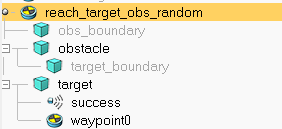
\includegraphics[scale=0.5]{assets/early-work/obs-random-scene-hierarchy.png}
    \caption{`ReachObs\_Random' Scene Hierarchy}
  \end{subfigure}
  \hfill
  \begin{subfigure}{0.45\linewidth}
    \centering
    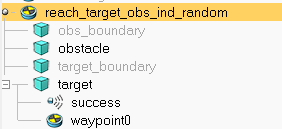
\includegraphics[scale=0.5]{assets/early-work/obs-ind-random-scene-hierarchy.png}
    \caption{`ReachObs\_IndRandom' Scene Hierarchy}
  \end{subfigure}
  \caption{Reaching Task with an Obstacle}\label{fig:reach-obs-random}
\end{figure}


\subsubsection{Wrist Camera Alone isn't Enough}

As expected, this is where the single wrist camera started showing its shortcomings. 

\todo{add graph of going around the obstacle but not quite reaching the target (wrist)}
\todo{show this with other combinations of cameras, comment on if the l/r without wrist can learn to go around the obstacle easily? maybe not, generalisation might be hard with no wrist}

The agent would easily move around the obstacle, however, would struggle to make the last steps in touching the target. This is mostly due to the fact that the demonstrations (which are provided by RlBench) are not necessarily pointing the wrist of the robot and hence the camera mounted there to look towards the target. This means that the wrist camera alone does not necessarily move towards the target, rather the robot learns to move behind the obstacle and nothing else.

From experiments I have realised that it learns to move around the obstacle easily, using simple behavioural cloning. However, getting the last nudge to actually reach the target is where it falls apart, especially in more realistic scenarios where the target is randomised behind the obstacle.

\subsubsection{Other Cameras}
Introducing the other cameras placed around in the environment, such as the \verb|left shoulder| or the \verb|right shoulder| cameras we can confirm that the wrist camera alone is not sufficient \todo{insert figure here with wrist vs others }, and the combination of wrist and other cameras are almost always the best as more coverage of the workspace guarantees less occlusions and more information the agent can work with to make decisions. It was clear that the wrist camera alone wasn't going to cut it unless it learnt to look towards the target.

\subsubsection{Implementing `Looking' into the Demonstrations}\todo{haven't done this yet}\label{ew-looking-at-target}
issues this is not easy might be working on this as a part of approach 2 later

Another way to make sure agent understands to look at the target is teaching it to actively seek out its target, either following previous works such as \todo{find some prior info tracking works add ref} or with attention mechanisms that figure out what is important in a task without prior object information \todo{maybe reference this later}

\section{Expanding the Task Space: Grasping Tasks}
Another task which is likely to suffer from lack of viewpoints is a grasping task. So I designed these tasks around the idea of grasping. Firstly, a simple version (Figure \ref{fig:grasp-simple}) which the agent learns to reach then grasp the cubic target. 

Main differences between this and the reaching task is that the target here is tangible, so on top of being rendered it is also set to be \emph{collidable}. Another major addition is the usage of the \emph{extension string} as seen in \ref{subfig:simple-zoom-actions}, this instructs the demonstration engine to insert certain moves within the movement of the simple trajectory. In this case \verb|open_gipper()| ensures the gripper is open, then a later waypoint will instruct it to close.

\todo{maybe some experiment resutls here?}

The more complicated counterpart, shown in Figure \ref{fig:grasp-move}, is a scenario where the cube needs to be picked up then moved to the target location (designated in green)

\begin{figure}[htpb] % htpb allows all placement
  \centering
  \begin{subfigure}{0.3\linewidth}
    \centering
    \includegraphics[scale=0.2]{../fyp/assets/task-pics/grasp/simple-front.png}
    \caption{Front}\label{subfig:simple-front}
  \end{subfigure}
  \hfill
  \begin{subfigure}{0.5\linewidth}
    \centering
    \includegraphics[scale=0.3]{../fyp/assets/task-pics/grasp/simple-front-zoom-gripper_actions.png}
    \caption{Zoomed, with gripper action}\label{subfig:simple-zoom-actions}
  \end{subfigure}
  \caption{Simple Grasping Task}\label{fig:grasp-simple}
\end{figure}

\begin{figure}[htpb] % htpb allows all placement
  \centering
  \begin{subfigure}{0.45\linewidth}
    \centering
    \includegraphics[scale=0.2]{../fyp/assets/task-pics/grasp/move-front.png} 
    \caption{Front}\label{subfig:grasp-move-front}
  \end{subfigure}
  \hfill
  \begin{subfigure}{0.45\linewidth}
    \centering
    \includegraphics[scale=0.2]{../fyp/assets/task-pics/grasp/move-top.png}
    \caption{Top}\label{subfig:grasp-move-top}
  \end{subfigure}
  \caption{Grasping then moving}\label{fig:grasp-move}
\end{figure}



\missingfigure{grasp pic and possibly the demo gifs}
\todo{add a picture with the cube grasped and the wrist camera view seen at that point}
Although, initially the wrist camera shouldn't pose any problems, as we advance through the task, especially after we have grasped something the wrist mounted camera becomes heavily obstructed and becomes unreliable so basing our decisions on this medium alone is not ideal.

\subsubsection{Observations}
What I got from these experiments was that the agent can benefit from understanding its surroundings at a higher level and more importantly remembering them. This is because once the camera becomes obstructed, as with \emph{Grasp Then Move}, even if the agent could do some exploration to find the target, it wouldn't be ideal due to the restricted view it has access to. So, observing the environment before, and remembering important parts will be vital for the later stages of tasks. I aim to explore some pre-policy visual exploration of the environment to be albe to address issues such as this one.
